\unnumberedChapter{Turnout Extension Board}

// ??? to do ....


\unnumberedSection{Block Diagram}

\begin{figure}[htbp]
    \centering
    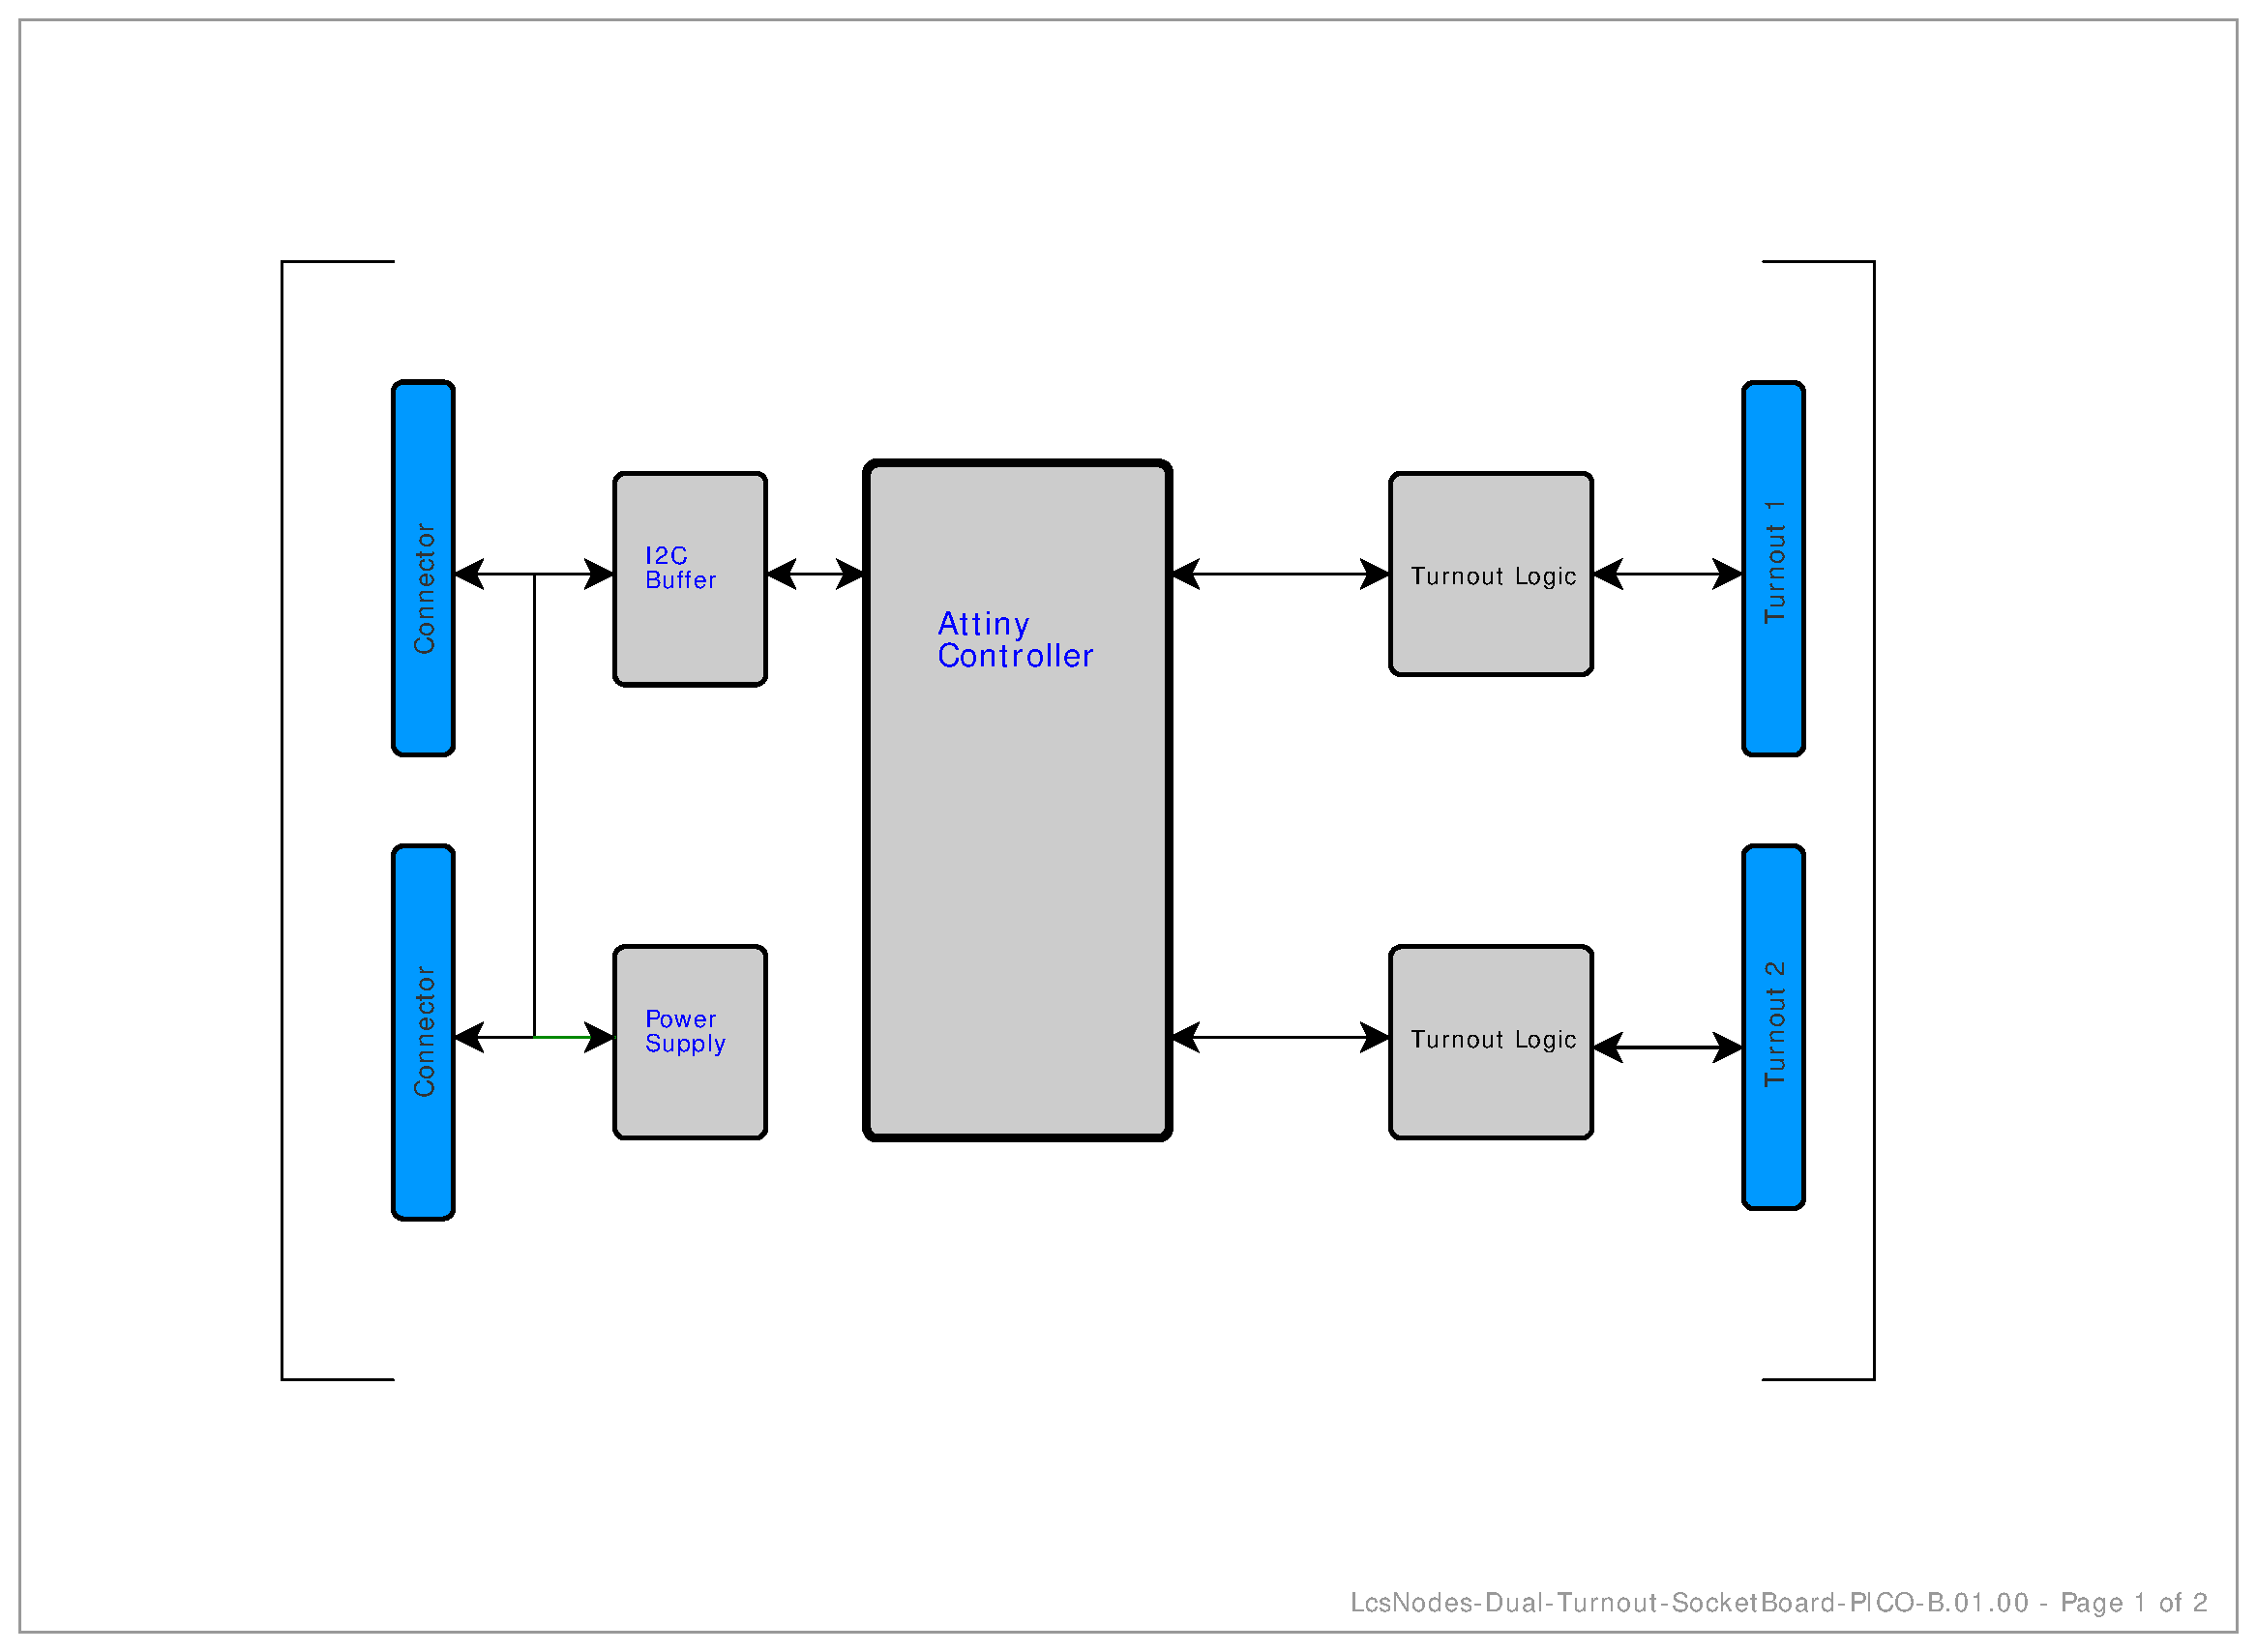
\includegraphics[page=1, width=0.9\textwidth]{./part-extensions/chapter-extension-turnouts/Schematic_LcsNodes-Dual-Turnout-Socket-Board.pdf}
\end{figure}
\FloatBarrier


\unnumberedSection{Logic}

- familiar Attiny / I2C concept for extensions

- use of bi stable relays, so we do not need too much energy after they switched.

- LEDs to see the state when you are lying underneath the layout


\begin{figure}[htbp]
    \centering
    \includegraphics[page=2, width=0.9\textwidth]{./part-extensions/chapter-extension-turnouts/Schematic_LcsNodes-Dual-Turnout-Socket-Board.pdf}
\end{figure}
\FloatBarrier


\unnumberedSection{PCB}

\begin{figure}[htbp]
    \centering
    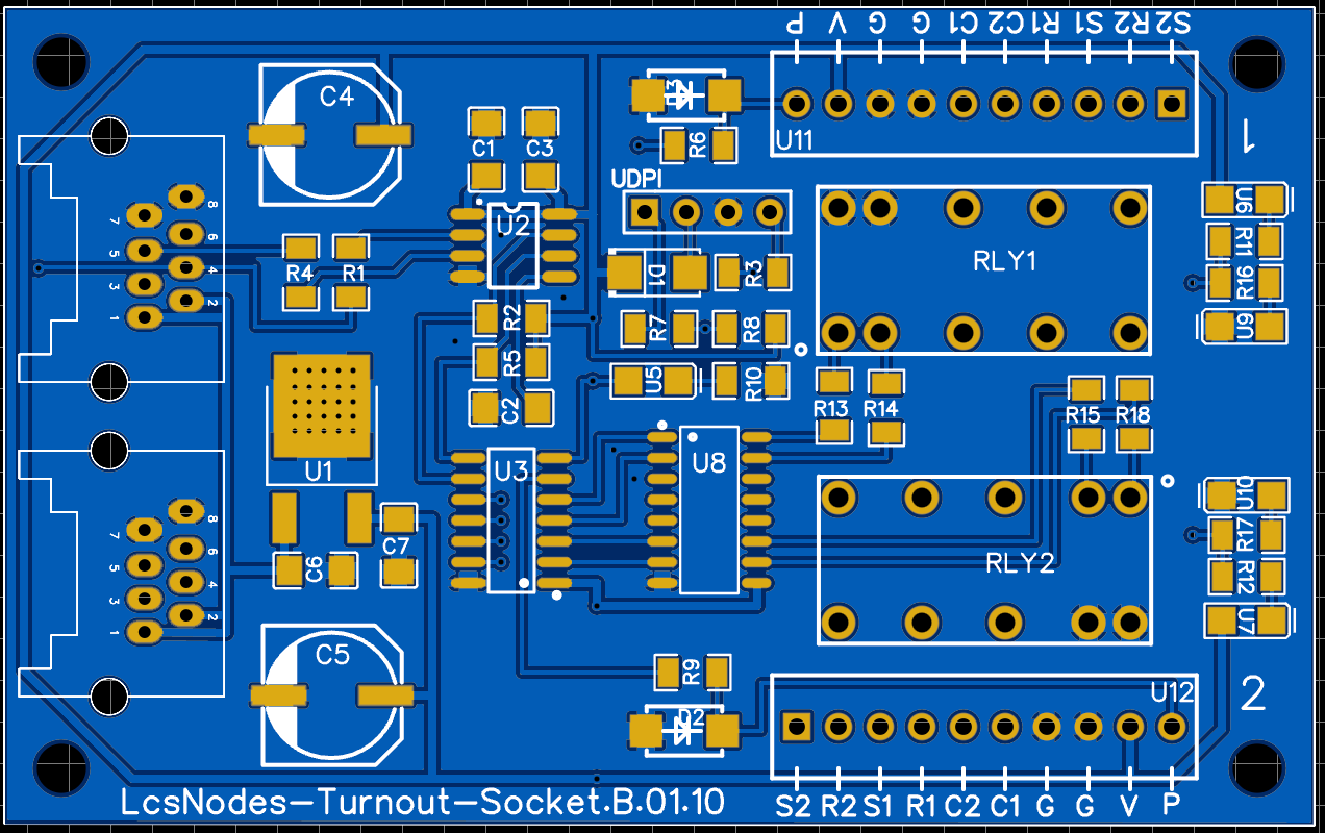
\includegraphics[page=1, width=0.7\textwidth]{./part-extensions/chapter-extension-turnouts/PCB_LcsNodes-Dual-Turnout-Socket-Board.pdf}
\end{figure}
\FloatBarrier

\unnumberedSection{Firmware}


\unnumberedSection{Summary}

// ??? quite a few parts, but a nice abstraction ...


